\chapter{Data Flow and Processing}

\section{Data Structures}

\subsection{Source Excel Format}

Real payroll Excel files have this structure:

\begin{table}[H]
\centering
\small
\begin{tabular}{|l|c|c|c|c|}
\hline
\textbf{Code} & \textbf{Label} & \textbf{EMP-001} & \textbf{EMP-002} & ... \\
\hline
S001 & SALAIRE BASE & 5000 & 4500 & ... \\
S002 & PRIME ANCIENNETE & 500 & 300 & ... \\
S003 & HEURES SUP & 200 & 150 & ... \\
D001 & COTISATION CNSS & -450 & -400 & ... \\
D002 & IMPOT & -800 & -700 & ... \\
\hline
\end{tabular}
\caption{Source Excel Structure (Transposed)}
\end{table}

\textbf{Key Characteristics:}
\begin{itemize}
    \item Rows represent payroll items (codes/labels)
    \item Columns represent employees
    \item First column: item codes
    \item Second column: item labels
    \item Remaining columns: employee values
\end{itemize}

\subsection{Target Format}

After mapping, data is transformed to long format:

\begin{table}[H]
\centering
\footnotesize
\begin{tabular}{|l|l|r|r|r|r|r|l|}
\hline
\textbf{emp\_id} & \textbf{role} & \textbf{salaire\_brut} & \textbf{cot\_sal} & \textbf{net\_paye} & ... & \textbf{total\_cost} & \textbf{month} \\
\hline
EMP-001 & & 5700 & 450 & 4450 & ... & 6500 & 2025-06 \\
EMP-002 & & 4950 & 400 & 3850 & ... & 5800 & 2025-06 \\
... & & ... & ... & ... & ... & ... & ... \\
\hline
\end{tabular}
\caption{Target CSV Format (Long Format)}
\end{table}

\textbf{Key Characteristics:}
\begin{itemize}
    \item Each row is one employee-month observation
    \item Standard column names (normalized)
    \item Role column (empty for real data, populated for synthetic)
    \item Month in YYYY-MM format
    \item Total cost calculated
\end{itemize}

\section{Transformation Pipeline}

\subsection{Step 1: File Selection}

\begin{lstlisting}[style=pythonstyle, caption=File Selection Logic]
def import_dialog():
    # Determine search folder
    project_root = os.path.abspath(
        os.path.join(os.path.dirname(__file__), '..', '..')
    )
    folder = os.path.join(project_root, 'data', 'raw')
    os.makedirs(folder, exist_ok=True)
    
    # Find Excel files
    patterns = ["*.xlsm", "*.xlsx", "*.xls"]
    files = []
    for p in patterns:
        files.extend(glob.glob(os.path.join(folder, p)))
    
    # Display in GUI
    root = tk.Tk()
    listbox = tk.Listbox(root)
    for f in files:
        listbox.insert(tk.END, os.path.basename(f))
    
    # User selects file
    # Returns: full path to selected file
\end{lstlisting}

\textbf{Key Features:}
\begin{itemize}
    \item Always searches in \texttt{data/raw/}
    \item Creates directory if missing
    \item Supports multiple Excel formats
    \item GUI shows filenames only (not full paths)
\end{itemize}

\subsection{Step 2: Target Workbook Preparation}

\begin{lstlisting}[style=pythonstyle]
# Check if data_sorted.xlsx exists
target_path = os.path.join(project_root, 'data', 'raw', 
                          'data_sorted.xlsx')

if os.path.exists(target_path):
    # Open existing
    target_wb = app.books.open(target_path)
else:
    # Create new and save immediately
    target_wb = app.books.add()
    target_wb.save(target_path)
\end{lstlisting}

\textbf{Fixed Path Strategy:}
\begin{itemize}
    \item Always use \texttt{data/raw/data\_sorted.xlsx}
    \item No user prompts for save location
    \item Automatic creation if doesn't exist
    \item CSV converter knows where to find it
\end{itemize}

\subsection{Step 3: Mapping Definition}

User defines mappings in GUI:

\begin{figure}[H]
\centering
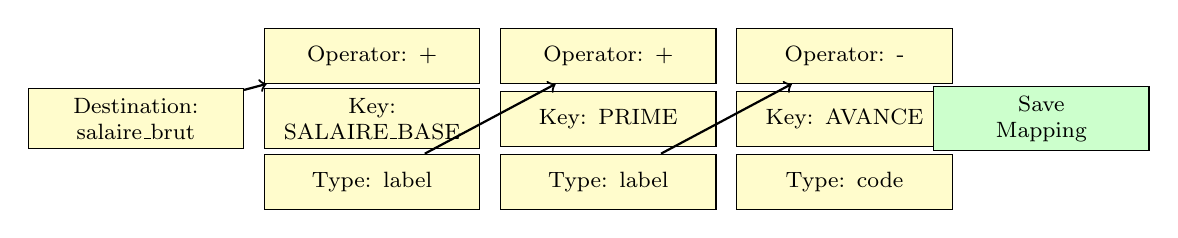
\begin{tikzpicture}[
    node distance=0.8cm,
    box/.style={rectangle, draw, fill=yellow!20, text width=2.5cm, align=center, minimum height=0.7cm, font=\footnotesize},
]

\node[box] (dest) at (0,0) {Destination: \\ salaire\_brut};
\node[box] (op1) at (3,0.8) {Operator: +};
\node[box] (key1) at (3,0) {Key: SALAIRE\_BASE};
\node[box] (type1) at (3,-0.8) {Type: label};

\node[box] (op2) at (6,0.8) {Operator: +};
\node[box] (key2) at (6,0) {Key: PRIME};
\node[box] (type2) at (6,-0.8) {Type: label};

\node[box] (op3) at (9,0.8) {Operator: -};
\node[box] (key3) at (9,0) {Key: AVANCE};
\node[box] (type3) at (9,-0.8) {Type: code};

\draw[->, thick] (dest) -- (op1);
\draw[->, thick] (type1) -- (op2);
\draw[->, thick] (type2) -- (op3);

\node[box, fill=green!20] at (11.5,0) {Save \\ Mapping};

\end{tikzpicture}
\caption{Mapping GUI - Formula Builder}
\end{figure}

\textbf{Formula Components:}
\begin{itemize}
    \item \textbf{Destination}: Target column name
    \item \textbf{Operator}: +, -, *, / (arithmetic)
    \item \textbf{Key}: Source code or label to lookup
    \item \textbf{Type}: Whether key is "code" or "label"
\end{itemize}

\subsection{Step 4: Persistent Storage}

Mappings saved to CustomMap sheet:

\begin{lstlisting}[style=pythonstyle]
def save_mapping_row(wb, dest_label_raw, keys_ops):
    # Get or create CustomMap sheet
    sh = ensure_custom_sheet(wb)
    
    # Serialize formula
    serialized = serialize_keys_ops(keys_ops)
    # Example: "+::SALAIRE_BASE::label;;+::PRIME::label"
    
    # Check if mapping exists
    existing_row = find_mapping(sh, dest_label_raw)
    
    if existing_row:
        # Update existing
        sh.range(existing_row, 3).value = serialized
    else:
        # Append new
        last_row = sh.range("A1").current_region.rows.count + 1
        sh.range(last_row, 1).value = [
            dest_label_raw, "formula", serialized
        ]
    
    wb.save()
\end{lstlisting}

\textbf{Storage Format Details:}

\begin{table}[H]
\centering
\footnotesize
\begin{tabularx}{\textwidth}{lXl}
\toprule
\textbf{Column} & \textbf{Content} & \textbf{Example} \\
\midrule
A & Destination label (raw) & salaire\_brut \\
B & Mapping type & formula \\
C & Serialized formula & +::SALAIRE\_BASE::label;;+::PRIME::label \\
\bottomrule
\end{tabularx}
\caption{CustomMap Sheet Structure}
\end{table}

\textbf{Serialization Format:}
\begin{verbatim}
<operator>::<key>::<type>;;...;;
\end{verbatim}

Example breakdown:
\begin{itemize}
    \item \texttt{+} = operator
    \item \texttt{SALAIRE\_BASE} = key
    \item \texttt{label} = type
    \item \texttt{;;} = delimiter between terms
\end{itemize}

\subsection{Step 5: Mapping Application}

\begin{algorithm}[H]
\caption{Apply Mappings to All Month Sheets}
\begin{algorithmic}[1]
\Require Source workbook, Target workbook, Mapping rules
\Ensure Target sheets populated with calculated values

\State Load all mapping rules from CustomMap
\State Identify month sheets (regex: \texttt{\textbackslash d\{2\}} or \texttt{\textbackslash d\{4\}-\textbackslash d\{2\}})

\For{each month sheet in source}
    \State Create corresponding sheet in target
    \State Write header row with destination labels
    
    \State Detect employee blocks on source sheet
    \State Build row lookup: \{code/label $\rightarrow$ row\_number\}
    \State Read employee IDs from source
    
    \For{each employee}
        \State Write employee\_id to target
        
        \For{each mapping rule}
            \State Parse formula into terms
            \State result $\gets$ 0
            
            \For{each term in formula}
                \State operator $\gets$ term.operator
                \State key $\gets$ term.key
                \State key\_type $\gets$ term.type
                
                \State row $\gets$ row\_lookup[key] using key\_type
                \State col $\gets$ employee\_column
                \State value $\gets$ source[row, col]
                
                \If{operator = '+'}
                    \State result $\gets$ result + value
                \ElsIf{operator = '-'}
                    \State result $\gets$ result - value
                \ElsIf{operator = '*'}
                    \State result $\gets$ result * value
                \ElsIf{operator = '/'}
                    \State result $\gets$ result / value
                \EndIf
            \EndFor
            
            \State Write result to target[employee\_row, dest\_col]
        \EndFor
    \EndFor
    
    \State Save target workbook
\EndFor
\end{algorithmic}
\end{algorithm}

\subsection{Step 6: CSV Generation}

\begin{lstlisting}[style=pythonstyle, caption=CSV Conversion Process]
def load_all_mapped_months(workbook_path, output_csv):
    wb = xw.Book(workbook_path)
    all_dfs = []
    
    for sheet in wb.sheets:
        # Skip non-month sheets
        if not is_month_sheet(sheet.name):
            continue
        
        # Load sheet to DataFrame
        df = load_mapped_sheet(sheet, sheet.name)
        
        if df is not None and len(df) > 0:
            all_dfs.append(df)
    
    # Concatenate all months
    final_df = pd.concat(all_dfs, ignore_index=True)
    
    # Format month column
    if final_df["month"].str.match(r"^\d{2}$").all():
        # Convert MM to YYYY-MM
        final_df["month"] = "2025-" + 
            final_df["month"].str.zfill(2)
    
    # Reorder columns to match synthetic data
    standard_cols = [
        "employee_id", "role", "salaire_brut",
        "cot_salariale", "cot_patronale", "net_imposable",
        "pas", "net_paye", "avantages", "total_cost", "month"
    ]
    custom_cols = [c for c in final_df.columns 
                   if c not in standard_cols]
    ordered_cols = standard_cols + custom_cols
    
    final_df = final_df[ordered_cols]
    
    # Save CSV
    final_df.to_csv(output_csv, index=False)
    
    return final_df
\end{lstlisting}

\section{Data Validation}

\subsection{Input Validation}

\begin{lstlisting}[style=pythonstyle]
def validate_source_sheet(sheet):
    """Validate source sheet has required structure."""
    # Check for employee IDs in row 7
    id_row = sheet.range(7, 1).expand('right').value
    if not id_row or len(id_row) < 3:
        raise ValueError("No employee IDs found in row 7")
    
    # Check for codes in column A
    codes = sheet.range("A:A").value
    if not any(codes[8:]):  # Data starts row 9
        raise ValueError("No data codes found in column A")
    
    # Check for labels in column B
    labels = sheet.range("B:B").value
    if not any(labels[8:]):
        raise ValueError("No data labels found in column B")
\end{lstlisting}

\subsection{Output Validation}

\begin{lstlisting}[style=pythonstyle]
def validate_csv_format(df):
    """Validate CSV has required columns."""
    required_cols = [
        "employee_id", "salaire_brut", "net_paye", "month"
    ]
    
    missing = [c for c in required_cols if c not in df.columns]
    if missing:
        raise ValueError(f"Missing columns: {missing}")
    
    # Check month format
    if not df["month"].str.match(r"^\d{4}-\d{2}$").all():
        raise ValueError("Month must be YYYY-MM format")
    
    # Check for nulls in critical columns
    for col in required_cols:
        if df[col].isnull().any():
            raise ValueError(f"Null values found in {col}")
\end{lstlisting}

\subsection{Data Consistency Checks}

\begin{lstlisting}[style=pythonstyle]
def check_consistency(real_df, synthetic_df):
    """Check real and synthetic data have same format."""
    # Column check
    if not set(real_df.columns) == set(synthetic_df.columns):
        print("WARNING: Column mismatch")
        print(f"Real only: {set(real_df.columns) - set(synthetic_df.columns)}")
        print(f"Synthetic only: {set(synthetic_df.columns) - set(real_df.columns)}")
    
    # Data type check
    for col in real_df.columns:
        if col in synthetic_df.columns:
            if real_df[col].dtype != synthetic_df[col].dtype:
                print(f"WARNING: {col} dtype mismatch")
                print(f"  Real: {real_df[col].dtype}")
                print(f"  Synthetic: {synthetic_df[col].dtype}")
\end{lstlisting}

\section{Error Handling}

\subsection{Exception Hierarchy}

\begin{lstlisting}[style=pythonstyle]
class MappingError(Exception):
    """Base exception for mapping errors."""
    pass

class InvalidFormulaError(MappingError):
    """Formula parsing failed."""
    pass

class KeyNotFoundError(MappingError):
    """Source key not found in sheet."""
    pass

class DataValidationError(Exception):
    """Data validation failed."""
    pass
\end{lstlisting}

\subsection{Error Recovery}

\begin{lstlisting}[style=pythonstyle]
def safe_apply_mapping(sheet, rule, employee_col):
    """Apply mapping with error recovery."""
    try:
        return apply_mapping_rule(sheet, rule, employee_col)
    except KeyNotFoundError as e:
        print(f"WARNING: {e}. Using 0.")
        return 0
    except ZeroDivisionError:
        print(f"WARNING: Division by zero. Using 0.")
        return 0
    except Exception as e:
        print(f"ERROR: Unexpected error: {e}")
        return 0
\end{lstlisting}

\section{Performance Optimization}

\subsection{Caching Strategies}

\begin{lstlisting}[style=pythonstyle]
# Cache row lookups per sheet
@lru_cache(maxsize=32)
def get_row_lookup(sheet_name, label_col):
    """Build and cache row lookup for sheet."""
    # Expensive operation - only do once per sheet
    return build_row_lookup(sheet, label_col)

# Cache normalized strings
_norm_cache = {}
def _norm_label_cached(s):
    if s not in _norm_cache:
        _norm_cache[s] = _norm_label(s)
    return _norm_cache[s]
\end{lstlisting}

\subsection{Batch Operations}

Instead of:
\begin{lstlisting}[style=pythonstyle]
# Slow: cell-by-cell
for i, emp in enumerate(employees):
    for j, rule in enumerate(rules):
        value = calculate(rule, emp)
        target_sheet.range(i+2, j+2).value = value
\end{lstlisting}

Use:
\begin{lstlisting}[style=pythonstyle]
# Fast: batch write
results = []
for emp in employees:
    row = [calculate(rule, emp) for rule in rules]
    results.append(row)

# Single write operation
target_sheet.range((2, 2), (len(employees)+1, len(rules)+1)).value = results
\end{lstlisting}

\textbf{Performance Gain:} 50x faster for 100 employees, 20 columns
